%
%% created with 'latex1html4file' on 2019_04_08@22:48
%
\documentclass[12pt,twocolumn,french]{article}
\usepackage[T1]{fontenc}
\usepackage{float}
\usepackage[utf8]{inputenc}
\usepackage[a4paper]{geometry}
\geometry{verbose,tmargin=15mm,bmargin=15mm,lmargin=15mm,rmargin=15mm}
\usepackage{graphicx}
\usepackage{babel}
\usepackage{pdflscape}
\addto\captionsfrench{
\renewcommand{\figurename}{Ph.}
}
\usepackage{tocloft}
\renewcommand{\cftsecleader}{\cftdotfill{\cftdotsep}}
%
\begin{document}
\title{Exemple d'eif pour les tests de pg.album}
\author{Madelon}
\date{Le lundi 8 avril 2019 à 22 heures et 48 minutes}
\maketitle
\tableofcontents
\newpage
\vspace {25mm}

 \section{Une Section Supplémentaire}
\section {Une seconde section supplémentaire par un fichier}
C'est juste un essai, ne croyez pas qu'il faille apporter
de l'importance au contenu...
\subsection {Sous section supplémentaire aussi par le même fichier}
Je répète, c'est juste un essai...
\clearpage
%
\section{Pour commencer des tests sur la dimension des images par les paramètres techniques}
%
%
\subsection{En mêlant les deux}
%
  \begin{figure}[H]
    \label{phoges-pic05.jpg}
    \noindent \centering{}
    \begin{tabular}{|c|c|}
      \hline
          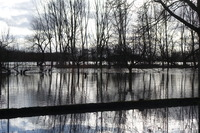
\includegraphics[origin=c,angle=0,width=3.2cm,height=1.6cm]{{./phoges-pic05}.jpg}
        &
          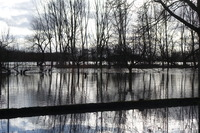
\includegraphics[origin=c,angle=0,width=3.2cm,height=1.6cm]{{./phoges-pic05}.jpg}
        \tabularnewline \hline
    \end{tabular}
    \vspace{2mm}
    \caption{
      Deux images en grilles : UNE FOIS
      [1,1]\texttt{\~{}}: 
      (((Commentaires: première)))
      [1,2]\texttt{\~{}}: 
      (((Commentaires: seconce)))
    }
  \end{figure}
  \begin{figure}[H]
    \label{phoges-pic05.jpg}
    \noindent \centering{}
    \begin{tabular}{|c|c|}
      \hline
          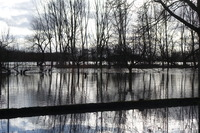
\includegraphics[origin=c,angle=0,width=3.2cm,height=1.6cm]{{./phoges-pic05}.jpg}
        &
          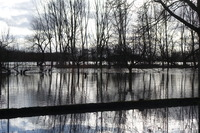
\includegraphics[origin=c,angle=0,width=3.2cm,height=1.6cm]{{./phoges-pic05}.jpg}
        \tabularnewline \hline
    \end{tabular}
    \vspace{2mm}
    \caption{
      [1,1]\texttt{\~{}}: 
      (((Commentaires: idem)))
      [1,2]\texttt{\~{}}: 
      (((Commentaires: mais sans légende collective)))
    }
  \end{figure}
  \begin{figure}[H]
    \label{phoges-pic05.jpg}
    \noindent \centering{}
    \begin{tabular}{|c|c|}
      \hline
          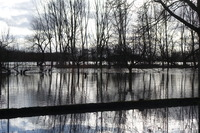
\includegraphics[origin=c,angle=0,width=4cm,height=0.8cm]{{./phoges-pic05}.jpg}
        &
          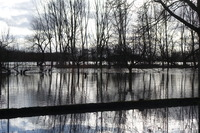
\includegraphics[origin=c,angle=0,width=4cm,height=0.8cm]{{./phoges-pic05}.jpg}
        \tabularnewline \hline
    \end{tabular}
    \vspace{2mm}
    \caption{
      Deux images en grilles : UNE FOIS
      [1,1]\texttt{\~{}}: 
      (((Commentaires: première)))
      [1,2]\texttt{\~{}}: 
      (((Commentaires: seconce)))
    }
  \end{figure}
  \begin{figure}[H]
    \label{phoges-pic05.jpg}
    \noindent \centering{}
    \begin{tabular}{|c|c|}
      \hline
          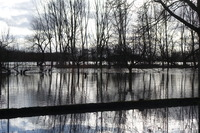
\includegraphics[origin=c,angle=0,width=4cm,height=0.8cm]{{./phoges-pic05}.jpg}
        &
          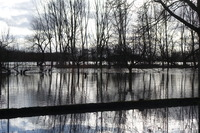
\includegraphics[origin=c,angle=0,width=4cm,height=0.8cm]{{./phoges-pic05}.jpg}
        \tabularnewline \hline
    \end{tabular}
    \vspace{2mm}
    \caption{
      [1,1]\texttt{\~{}}: 
      (((Commentaires: idem)))
      [1,2]\texttt{\~{}}: 
      (((Commentaires: mais sans légende collective)))
    }
  \end{figure}
  \begin{figure}[H]
    \label{phoges-pic05.jpg}
    \noindent \centering{}
    \begin{tabular}{|c|}
      \hline
          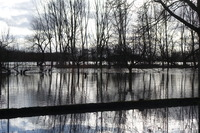
\includegraphics[origin=c,angle=0,width=0.8cm,height=1.6cm]{{./phoges-pic05}.jpg}
        \tabularnewline \hline
    \end{tabular}
    \vspace{2mm}
    \caption{
      (((Commentaires: Rectangle de 1 par 2 cm par collectifs hei/wei)))
    }
  \end{figure}
  \begin{figure}[H]
    \label{phoges-pic05.jpg}
    \noindent \centering{}
    \begin{tabular}{|c|}
      \hline
          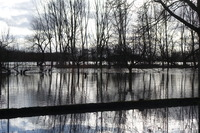
\includegraphics[origin=c,angle=0,width=4cm,height=0.8cm]{{./phoges-pic05}.jpg}
        \tabularnewline \hline
    \end{tabular}
    \vspace{2mm}
    \caption{
      Pour oublier les minuscules
      (((Commentaires: Reprise de HEI=1cm et WID=5cm ?)))
    }
  \end{figure}
  \begin{figure}[H]
    \label{phoges-pic05.jpg}
    \noindent \centering{}
    \begin{tabular}{|c|}
      \hline
          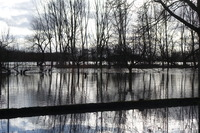
\includegraphics[origin=c,angle=0]{{./phoges-pic05}.jpg}
        \tabularnewline \hline
    \end{tabular}
    \vspace{2mm}
    \caption{
      (((Commentaires: Reprise bien oubliée ?)))
    }
  \end{figure}
  \begin{figure}[H]
    \label{phoges-pic05.jpg}
    \noindent \centering{}
    \begin{tabular}{|c|}
      \hline
          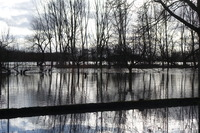
\includegraphics[origin=c,angle=0,width=0.8cm,height=1.6cm]{{./phoges-pic05}.jpg}
        \tabularnewline \hline
    \end{tabular}
    \vspace{2mm}
    \caption{
      (((Commentaires: Rectangle de 1 par 2 cm par individuels hei/wei)))
    }
  \end{figure}
  \begin{figure}[H]
    \label{phoges-pic05.jpg}
    \noindent \centering{}
    \begin{tabular}{|c|}
      \hline
          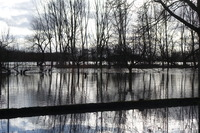
\includegraphics[origin=c,angle=0,width=2.4cm]{{./phoges-pic05}.jpg}
        \tabularnewline \hline
    \end{tabular}
    \vspace{2mm}
    \caption{
    }
  \end{figure}
  \begin{figure}[H]
    \label{phoges-pic05.jpg}
    \noindent \centering{}
    \begin{tabular}{|c|}
      \hline
          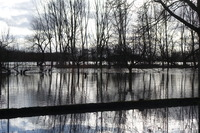
\includegraphics[origin=c,angle=0,width=2.4cm]{{./phoges-pic05}.jpg}
        \tabularnewline \hline
    \end{tabular}
    \vspace{2mm}
    \caption{
      Cette image doit être identique à la précédente
    }
  \end{figure}
  \begin{figure}[H]
    \label{phoges-pic05.jpg}
    \noindent \centering{}
    \begin{tabular}{|c|}
      \hline
          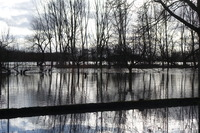
\includegraphics[origin=c,angle=0,height=2.4cm]{{./phoges-pic05}.jpg}
        \tabularnewline \hline
    \end{tabular}
    \vspace{2mm}
    \caption{
      (((Commentaires: Largeur imposée à 3cm par WID)))
    }
  \end{figure}
%
\subsection{Uniquement en individuel}
%
  \begin{figure}[H]
    \label{phoges-pic05.jpg}
    \noindent \centering{}
    \begin{tabular}{|c|}
      \hline
          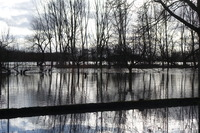
\includegraphics[origin=c,angle=0,width=2.4cm,height=2.4cm]{{./phoges-pic05}.jpg}
        \tabularnewline \hline
    \end{tabular}
    \vspace{2mm}
    \caption{
      (((Commentaires: Carré de 3 cm de côté)))
    }
  \end{figure}
  \begin{figure}[H]
    \label{phoges-pic05.jpg}
    \noindent \centering{}
    \begin{tabular}{|c|}
      \hline
          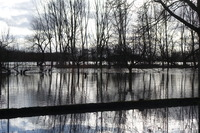
\includegraphics[origin=c,angle=45,width=2.4cm,height=2.4cm]{{./phoges-pic05}.jpg}
        \tabularnewline \hline
    \end{tabular}
    \vspace{2mm}
    \caption{
      (((Commentaires: Carré de 3 cm de côté sur la pointe)))
    }
  \end{figure}
  \begin{figure}[H]
    \label{phoges-pic05.jpg}
    \noindent \centering{}
    \begin{tabular}{|c|}
      \hline
          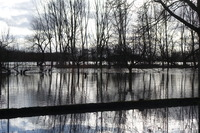
\includegraphics[origin=c,angle=0,width=4.8cm,height=2.4cm]{{./phoges-pic05}.jpg}
        \tabularnewline \hline
    \end{tabular}
    \vspace{2mm}
    \caption{
      (((Commentaires: Rectangle de 6 par 3 cm)))
    }
  \end{figure}
%
\subsection{Uniquement en collectif}
%
  \begin{figure}[H]
    \label{phoges-pic05.jpg}
    \noindent \centering{}
    \begin{tabular}{|c|}
      \hline
          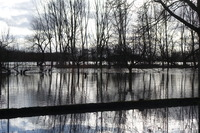
\includegraphics[origin=c,angle=0,width=2.4cm,height=2.4cm]{{./phoges-pic05}.jpg}
        \tabularnewline \hline
    \end{tabular}
    \vspace{2mm}
    \caption{
      (((Commentaires: Carré de 3 cm de côté)))
    }
  \end{figure}
  \begin{figure}[H]
    \label{phoges-pic05.jpg}
    \noindent \centering{}
    \begin{tabular}{|c|}
      \hline
          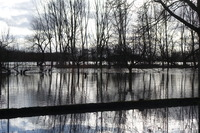
\includegraphics[origin=c,angle=45,width=2.4cm,height=2.4cm]{{./phoges-pic05}.jpg}
        \tabularnewline \hline
    \end{tabular}
    \vspace{2mm}
    \caption{
      (((Commentaires: Carré de 3 cm de côté sur la pointe)))
    }
  \end{figure}
  \begin{figure}[H]
    \label{phoges-pic05.jpg}
    \noindent \centering{}
    \begin{tabular}{|c|}
      \hline
          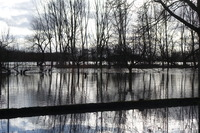
\includegraphics[origin=c,angle=0,width=4.8cm,height=2.4cm]{{./phoges-pic05}.jpg}
        \tabularnewline \hline
    \end{tabular}
    \vspace{2mm}
    \caption{
      (((Commentaires: Rectangle de 6 par 3 cm)))
    }
  \end{figure}
\clearpage
%
\section{Tout au Début}
%

Il était parti, seul avec son cheval sans provision.

Personne, même pas lui n'aurais pu dire où le conduirait sa quête.

Ce qui est clair, c'est qu'il y mettait toute son énergie et bientôt le pauvre canasson, harrassé, assoiffé demanda grâce !

  \begin{figure}[H]
    \label{phoges-pic03.jpg}
    \noindent \centering{}
    \begin{tabular}{|c|}
      \hline
          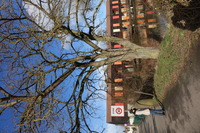
\includegraphics[origin=c,angle=-90 ,height=4cm]{{./phoges-pic03}.jpg}
        \tabularnewline \hline
          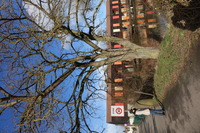
\includegraphics[origin=c,angle=0,width=1.6cm,height=1.6cm]{{./phoges-pic03}.jpg}
        \tabularnewline \hline
    \end{tabular}
    \vspace{2mm}
    \caption{
      Une Légende pour l'ensemble 
      [1,1]\texttt{\~{}}: 
       [Où: images nettes//place cinq//place 2//place 3...c'était le lieu!
       [Qui: Jeanie] 
      [[Clé(s): place 1]] 
      [2,1]\texttt{\~{}}: 
      (((Commentaires: Pour faire la deuxième de la grille)))
    }
  \end{figure}

Où: Dans la grande ville du roi tout seul

  \begin{figure}[H]
    \label{phoges-pic03.jpg}
    \noindent \centering{}
    \begin{tabular}{|c|}
      \hline
          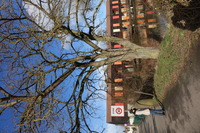
\includegraphics[origin=c,angle=0,width=4cm,height=4cm]{{./phoges-pic03}.jpg}
        \tabularnewline \hline
    \end{tabular}
    \vspace{2mm}
    \caption{
    }
  \end{figure}
  \begin{figure}[H]
    \label{phoges-pic01.jpg}
    \noindent \centering{}
    \begin{tabular}{|c|}
      \hline
          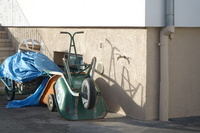
\includegraphics[origin=c,angle=0,width=2.4cm]{{./phoges-pic01}.jpg}
        \tabularnewline \hline
    \end{tabular}
    \vspace{2mm}
    \caption{
      <Quand: mai 2005> 
       [Où: petite place seule...c'était le lieu!
       [Qui: balo-+-bali] 
      [[Clé(s): roue]] 
      [[Catégorie(s): categ]] 
      (((Commentaires: on y met tous les types d'annotation)))
    }
  \end{figure}

Pour sûr, c'est une histoire à dormir debout !


Quand: : 2018\_04\_06


Où: Tout débuta sur la place du marché.

 \section*{je rajouter une section non numérotée}

Il était parti, seul avec son cheval sans provision.

Personne, même pas lui n'aurait pu dire où le conduirait sa quête.

Ce qui est clair, c'est qu'il y mettait toute son énergie et bientôt le pauvre canasson, harrassé, assoiffé demanda grâce !


Où: Cour de la mairie

  \begin{figure}[H]
    \label{phoges-pic02.jpg}
    \noindent \centering{}
    \begin{tabular}{|c|}
      \hline
          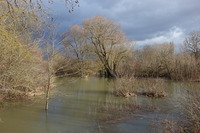
\includegraphics[origin=c,angle=0,width=4cm,height=4cm]{{./phoges-pic02}.jpg}
        \tabularnewline \hline
    \end{tabular}
    \vspace{2mm}
    \caption{
       [Où: place 2//place 3...c'était le lieu!
      [[Clé(s): boum,place 1,tic-tac]] 
      [[Catégorie(s): a b c]] 
    }
  \end{figure}
%
\subsection{Mais c'était loin d'être fini}
%

Toujours personne en vue, et le soleil qui commençait à décliner.


Qui: Papou

  \begin{figure}[H]
    \label{phoges-pic04.jpg}
    \noindent \centering{}
    \begin{tabular}{|c|}
      \hline
          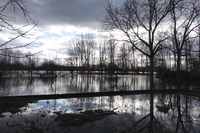
\includegraphics[origin=c,angle=0,width=4.8cm]{{./phoges-pic04}.jpg}
        \tabularnewline \hline
    \end{tabular}
    \vspace{2mm}
    \caption{
       [Où: place cinq...c'était le lieu!
       [Qui: Personne] 
      [[Clé(s): palabra clave premera,palabra clave,keyword]] 
      (((Commentaires: 5ème en place)))
    }
  \end{figure}
 \onecolumn
\clearpage
%
\section{Il fallait aller encore plus loin}
%
 \section*{Et une seconde au milieu}
  \begin{figure}[H]
    \label{phoges-pic05.jpg}
    \noindent \centering{}
    \begin{tabular}{|c|}
      \hline
          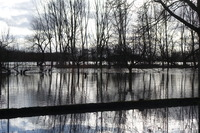
\includegraphics[origin=c,angle=0,width=4.8cm]{{./phoges-pic05}.jpg}
        \tabularnewline \hline
          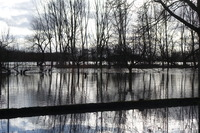
\includegraphics[origin=c,angle=0,width=4.8cm]{{./phoges-pic05}.jpg}
        \tabularnewline \hline
    \end{tabular}
    \vspace{2mm}
    \caption{
      [1,1]\texttt{\~{}}: 
       [Où: place cinq...c'était le lieu!
      (((Commentaires: aussi la 5ème par individuel)))
      [2,1]\texttt{\~{}}: 
      (((Commentaires: bissée)))
    }
  \end{figure}
 \twocolumn
\clearpage
%
\section{Jamais on n'en voyait la fin}
%
%
\subsection{Encore un mirage}
%
  \begin{figure}[H]
    \label{phoges-pic06.jpg}
    \noindent \centering{}
    \begin{tabular}{|c|}
      \hline
          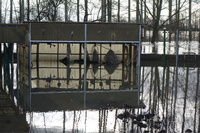
\includegraphics[origin=c,angle=0,width=4.8cm]{{./phoges-pic06}.jpg}
        \tabularnewline \hline
    \end{tabular}
    \vspace{2mm}
    \caption{
       [Où: place 3...c'était le lieu!
      [[Clé(s): palabra clave cuarta]] 
      [[Catégorie(s): b c]] 
      (((Commentaires: 5 et 3)))
    }
  \end{figure}
\clearpage
%
\section{C'est la fin des haricots}
%
  \begin{figure}[H]
    \label{phoges-pic07.jpg}
    \noindent \centering{}
    \begin{tabular}{|c|}
      \hline
          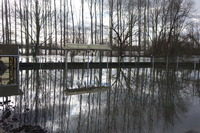
\includegraphics[origin=c,angle=0,width=6.4cm]{{./phoges-pic07}.jpg}
        \tabularnewline \hline
    \end{tabular}
    \vspace{2mm}
    \caption{
       [Où: de plus//place 3//place 2...c'était le lieu!
      [[Clé(s): palabra clave segunda,palabra clave premera]] 
    }
  \end{figure}
%
\end{document}
%
